\documentclass[aspectratio=169]{beamer}
\usetheme{Darmstadt}
\usepackage{graphicx}
\usepackage[ngerman]{babel}
\usepackage[T1]{fontenc}
\usepackage[utf8]{inputenc}
\usepackage{tikz}
\usepackage[shadow,colorinlistoftodos]{todonotes}
\setbeamertemplate{footline}[frame number]

\newcommand{\cc}[1]{\includegraphics[height=4mm]{img/#1.png}}
\usepackage{ifthen}
\newcommand{\license}[2][]{\\#2\ifthenelse{\equal{#1}{}}{}{\\\scriptsize\url{#1}}}
\usepackage{textcomp}

\usepackage{tikz}
\usetikzlibrary{positioning,arrows}

\tikzstyle{cell} = [rectangle, draw=black, fill=gray!20, minimum width=25pt]

\newcommand\code[2]{
  \centerline{
    \begin{tikzpicture}[transform shape]
      \draw [draw=white, very thick, ->] (0,0.8) -- (0,0.5);
      \foreach \value [count=\x] in {#1} {
        \draw (\x/2,0) node{$\value$};
      }
      \draw [very thick, ->] (#2/2,0.8) -- (#2/2,0.5);
    \end{tikzpicture}
  }
}

\newcommand\cells[2]{
  \centerline{
    \begin{tikzpicture}[transform shape]
      \foreach \value [count=\x] in {#1} {
        \draw (\x,0) node[cell]{$\value$};
      }
      \draw [very thick, ->] (#2,-0.8) -- (#2,-0.5);
    \end{tikzpicture}
  }
}

\newcommand\brainfuck[4]{
  \only<+>{
    \vspace{10pt}
    \code{#1}{#2}
    \vspace{10pt}
    \cells{#3}{#4}
    \vspace{10pt}
  }
}

%\setbeamercovered{transparent}


\title{Brainfuck}
\author{Thammi}
\date{21.09.2018}

\begin{document}
\maketitle

\begin{frame}[t]
	\frametitle{Konzept}
  \begin{itemize}
    \item<2-> Programmiersprache mit nur Acht Befehlen
    \item<3-> endloses Band mit Zahlen
    \item<4-> beweglicher Schreib- und Lesekopf
  \end{itemize}
  \only<5->{
    \cells{0,0,0,0,0,0,0,0}{1}
  }
\end{frame}

\begin{frame}[t]
	\frametitle{Rechenoperationen}
  \begin{itemize}
    \item '+' erhöht um eins
    \item '-' verringert um eins
  \end{itemize}

  \brainfuck{+,+,+,-}{0}{0,0,0,0,0,0,0,0}{1}
  \brainfuck{+,+,+,-}{1}{1,0,0,0,0,0,0,0}{1}
  \brainfuck{+,+,+,-}{2}{2,0,0,0,0,0,0,0}{1}
  \brainfuck{+,+,+,-}{3}{3,0,0,0,0,0,0,0}{1}
  \brainfuck{+,+,+,-}{4}{2,0,0,0,0,0,0,0}{1}
\end{frame}

\begin{frame}[t]
	\frametitle{Kopf bewegen}
  \begin{itemize}
    \item '<' bewegt nach links
    \item '>' bewegt nach rechts
  \end{itemize}

  \brainfuck{+,+,>,+,<,-}{0}{0,0,0,0,0,0,0,0}{1}
  \brainfuck{+,+,>,+,<,-}{1}{1,0,0,0,0,0,0,0}{1}
  \brainfuck{+,+,>,+,<,-}{2}{2,0,0,0,0,0,0,0}{1}
  \brainfuck{+,+,>,+,<,-}{3}{2,0,0,0,0,0,0,0}{2}
  \brainfuck{+,+,>,+,<,-}{4}{2,1,0,0,0,0,0,0}{2}
  \brainfuck{+,+,>,+,<,-}{5}{2,1,0,0,0,0,0,0}{1}
  \brainfuck{+,+,>,+,<,-}{6}{1,1,0,0,0,0,0,0}{1}
\end{frame}

\begin{frame}[t]
	\frametitle{Schleifen}
  \begin{itemize}
    \item '[' springt hinter das zugehörige ']' wenn aktuelle Zelle 0 ist
    \item ']' sprint zum zugehörigen '['
  \end{itemize}

  \brainfuck{[,-,>,+,<,]}{0}{3,0,0,0,0,0,0,0}{1}
  \brainfuck{[,-,>,+,<,]}{1}{3,0,0,0,0,0,0,0}{1}
  \brainfuck{[,-,>,+,<,]}{2}{2,0,0,0,0,0,0,0}{1}
  \brainfuck{[,-,>,+,<,]}{3}{2,0,0,0,0,0,0,0}{2}
  \brainfuck{[,-,>,+,<,]}{4}{2,1,0,0,0,0,0,0}{2}
  \brainfuck{[,-,>,+,<,]}{5}{2,1,0,0,0,0,0,0}{1}
  \brainfuck{[,-,>,+,<,]}{6}{2,1,0,0,0,0,0,0}{1}

  \brainfuck{[,-,>,+,<,]}{1}{2,1,0,0,0,0,0,0}{1}
  \brainfuck{[,-,>,+,<,]}{2}{1,1,0,0,0,0,0,0}{1}
  \brainfuck{[,-,>,+,<,]}{3}{1,1,0,0,0,0,0,0}{2}
  \brainfuck{[,-,>,+,<,]}{4}{1,2,0,0,0,0,0,0}{2}
  \brainfuck{[,-,>,+,<,]}{5}{1,2,0,0,0,0,0,0}{1}
  \brainfuck{[,-,>,+,<,]}{6}{1,2,0,0,0,0,0,0}{1}

  \brainfuck{[,-,>,+,<,]}{1}{1,2,0,0,0,0,0,0}{1}
  \brainfuck{[,-,>,+,<,]}{2}{0,2,0,0,0,0,0,0}{1}
  \brainfuck{[,-,>,+,<,]}{3}{0,2,0,0,0,0,0,0}{2}
  \brainfuck{[,-,>,+,<,]}{4}{0,3,0,0,0,0,0,0}{2}
  \brainfuck{[,-,>,+,<,]}{5}{0,3,0,0,0,0,0,0}{1}
  \brainfuck{[,-,>,+,<,]}{6}{0,3,0,0,0,0,0,0}{1}

  \brainfuck{[,-,>,+,<,]}{1}{0,3,0,0,0,0,0,0}{1}
\end{frame}

\begin{frame}[t]
	\frametitle{Ein- und Ausgabe}
  \begin{itemize}
    \item '.' gibt die aktuelle Zelle aus
    \item ',' liest in die aktuelle Zelle ein
  \end{itemize}

  \brainfuck{{,},+,.}{0}{0,0,0,0,0,0,0,0}{1}
  \brainfuck{{,},+,.}{1}{97,0,0,0,0,0,0,0}{1}
  \brainfuck{{,},+,.}{2}{98,0,0,0,0,0,0,0}{1}
  \brainfuck{{,},+,.}{3}{98,0,0,0,0,0,0,0}{1}
\end{frame}

\begin{frame}[t]
	\frametitle{Codeschnipsel}
  \begin{itemize}
    \item<+-> Verschieben
    \begin{itemize}
      \item<+-> {} [->+<]
    \end{itemize}
    \item<+-> Kopieren
    \begin{itemize}
      \item<+-> {} [->+>+<{}<][>{}>-<{}<+]
    \end{itemize}
    \item<+-> Multiplikation
    \begin{itemize}
      \item<+-> {} [->++++<]
      \item<+-> {} [->[->+>+<{}<]>{}>[-<{}<+>{}>]<{}<{}<]
    \end{itemize}
    \item<+-> Division
    \begin{itemize}
      \item<+-> {} [-{}-{}->+<]
    \end{itemize}
    \item<+-> Hello World
    \begin{itemize}
      \item<+-> {} +[-[<{}<[+[--->]-[<{}<{}<]]]>{}>{}>-]>-.---.>..>.<{}<{}<{}<-.<+.>{}>{}>{}>{}>.>.<{}<.<-.
    \end{itemize}
    \item<+-> Echo
    \begin{itemize}
      \item<+-> ,[.,]
    \end{itemize}
  \end{itemize}
\end{frame}

\begin{frame}[t]
	\frametitle{Pfadfinder}
  \only<2>{
    \centerline{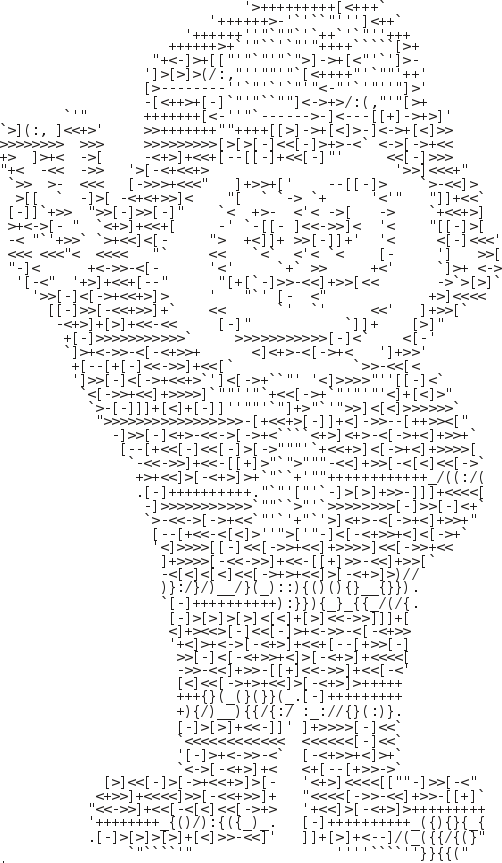
\includegraphics[height=0.8\textheight]{img/scout.png}}
  }
\end{frame}

\end{document}
